%-----------------------------------------------------------------------------
% Schriftgr��e, Layout, Papierformat, Art des Dokumentes
%-----------------------------------------------------------------------------
\documentclass[12pt,					% Grundschriftge
							 oneside,			% einseitiges Dokument
							 a4paper,			% Papiergr��e
							 halfparskip,		% Einzug bei einem Absatz
							 liststotoc,			% Verzeichniss (Abbildungen erc.) in das Inhaltverzeichnis
							 bibtotoc,			% Literaturverzeichnis ins Inhaltverzeichnis
							 fleqn,				% Mathematische Formeln linksb�ndig darstellen
							 pointlessnumbers]	% Punkt am Ende der Nummerierung des Inhaltsverzeichnisses 													entfernen
							 {scrreprt}

%-----------------------------------------------------------------------------
% Konstanten festlegen
%-----------------------------------------------------------------------------


\newcommand{\VerfasserJ}{Josef Prothmann}
\newcommand{\GeburtstagJ}{16. Dezember 1998}
\newcommand{\GeburtsortJ}{Dannenberg/ Elbe}
\newcommand{\EmailJ}{j.prothmann@stud.hs-wismar.de}

\newcommand{\VerfasserC}{Christoph Werner}
\newcommand{\GeburtstagC}{16. November 1993}
\newcommand{\GeburtsortC}{Fürth (bayern)}
\newcommand{\EmailC}{christoph.werner@stud.hs-wismar.de}


\newcommand{\Titel}{Data Mining Semesterprojekt Dokumentation}

\newcommand{\Betreuer}{Prof. Dr. rer. nat. Jürgen Cleve}


\newcommand{\blankpage}{
%	\newpage
%	\thispagestyle{empty}
%	\mbox{}
	\newpage
}

%-----------------------------------------------------------------------------
% verwendete Pakete
%-----------------------------------------------------------------------------
\usepackage[utf8]{inputenc}		% Zeichkodierung , Umlaute erlauben
\usepackage[T1]{fontenc}				% Wahl des Fonts, bzw. der Kodierung
\usepackage[english,ngerman]{babel}		% neue deutsche Rechtschreibung verwenden
\usepackage{graphicx}					% erm�glicht das Einbinden von Grafiken, sehr wichtig!
\usepackage{fancyhdr}					% f�r formatierte Kopf- und Fu�zeilen
\usepackage{setspace}					% Package zum Kontrollieren von Leerr�umen
\usepackage{subfigure}					% erweiterte Darstellung von Bildern
\usepackage{listings}					% M�glickeit zum Anzeigen von Quelltexten
\usepackage{color,moreverb}				% Farben
\usepackage{lmodern}					% bietet neuere Schriften, sieht besser aus im Acrobat Reader
\usepackage{amsmath,amssymb}			% erweiteter Formelsatz und zus�tzliche Mathe-Symbole
\usepackage{booktabs}					% professionelle, typographisch richtige Tabellen
\usepackage{cite}						% f�r LibTex
%\usepackage{shortvrb}					% f�r Quellcode mit \begin{verbatim}
%\usepackage[binary-units=true]{siunitx}	% Darstellung von Si-Einheiten
%\usepackage{pdfpages}					% pdf-Seiten einbinden
\usepackage{enumitem}					% custom itemiziation





%-----------------------------------------------------------------------------
% Fu�notennummerierung nicht f�r jedes kapitel zur�cksetzen
%-----------------------------------------------------------------------------
\usepackage{chngcntr}
\counterwithout{footnote}{chapter}

%-----------------------------------------------------------------------------
% Einstellungen der Seitenr�nder
%-----------------------------------------------------------------------------
\usepackage[left=3cm,						% linker Rand
						right=3cm,			% rechter Rand
						top=1.5cm,			% oberer Rand
						bottom=1.5cm,		% unterer Rand
						includeheadfoot,	% bezieht die Kopf- und Fu�zeile mit ein
						bindingoffset=0cm]	% Bundsteg
						{geometry}


%-----------------------------------------------------------------------------
% Daten f�r die Titel des Artikels
%-----------------------------------------------------------------------------
\title{Semesterarbeit Data Mining}
\author{\VerfasserC, \Verfasserj}
\date{\today{}}

%-----------------------------------------------------------------------------
% Metadaten in pdf einf�gen
%-----------------------------------------------------------------------------
\usepackage[pdftex,
						pdfauthor={\VerfasserC, \VerfasserJ},									% Name des Autors
						pdftitle={\Titel},										% Name der Arbeit
						pdfcreator={MiKTeX, LaTeX with hyperref and KOMA-Script},	% Von was erzeugt
						pdfsubject={Semesterarbeit Data Mining},							% Was f�r eine Arbeit ist es
						pdfkeywords={\Titel},
						plainpages=false,
						hypertexnames=false,
						pdfpagelabels]{hyperref}

%-----------------------------------------------------------------------------
% Schriftarten anpassen
%-----------------------------------------------------------------------------
\setkomafont{sectioning}{\rmfamily\bfseries}			% Titelzeilen
\setkomafont{caption}{\small}							% Schrift f�r Caption
\setkomafont{captionlabel}{\sffamily\bfseries\small}	% Schrift f�r 'Abbildung'
\setkomafont{chapterentry}{\small\bfseries}				% Schrift f�r Inhaltsverzeichnis
\setkomafont{chapter}{\large\bfseries}					% Schrift f�r Kapitel
\setkomafont{section}{\normalsize}						% Schrift f�r Section
\setkomafont{subsection}{\normalsize}					% Schrift f�r Subsection



%-----------------------------------------------------------------------------
% Farbe f�r Links in PDF-Dokumenten definieren
%-----------------------------------------------------------------------------
\definecolor{LinkColor}{rgb}{0,0,0}				% Festlegen einer neuen Farbe

\hypersetup{colorlinks=true,					% farbliche Links
						breaklinks=true,		% Zeilenumbruch erlauben
						linkcolor=black,		% Farbe f�r interne Links
						citecolor=black,		% Farbe f�r Links zum Literaturverzeichnis
						filecolor=LinkColor,	% Farbe f�r externe Dateilinks
						menucolor=LinkColor,	%
						urlcolor=LinkColor}		% Farbe f�r externe Links
						



				
%-----------------------------------------------------------------------------
% Kopf- und Fusszeile bestimmen
%-----------------------------------------------------------------------------
\pagestyle{fancy}	
\fancyhf{}												% alle Felder l�schen
\fancypagestyle{plain}{}

% Kopfzeile rechts bzw. au�en
\fancyhead[R]{\nouppercase{\leftmark}}
% Linie oben
\renewcommand{\headrulewidth}{0.5pt}
% Fu�zeile rechts bzw. au�en
\fancyfoot[R]{\thepage}
%-----------------------------------------------------------------------------

%-----------------------------------------------------------------------------
% Begin des Dokuments
%-----------------------------------------------------------------------------

\begin{document} 						% Beginn des Dokumentes

	\renewcommand\lstlistingname{Code}
	\renewcommand\lstlistlistingname{Codeverzeichnis}
	
	%% Titel
	\begin{titlepage}
		\setlength\headsep{-5mm}
		\begin{figure}[!h]
			\begin{minipage}{0.8\textwidth}
				\textbf{Hochschule Wismar} \\
				University of Applied Sciences \\
				Technology, Business and Design \\
				Fakultät für Ingenieurwissenschaften, Bereich EuI \\
			\rule{\textwidth}{0.5pt}
			\end{minipage}
			\begin{minipage}[r]{0.1\textwidth}
				\begin{flushright}
					
\includegraphics[height=6\baselineskip]{pictures/HS-Wismar_Logo-FIW_2010-01.jpg}
				\end{flushright}
			\end{minipage}
		\end{figure}
		\vspace*{6cm}
		\begin{center}
			\Huge
			\textbf{Semesterarbeit} \\
			\vspace{2cm}
			\large \Titel
			\begin{table*}[b]
				\begin{tabular}{rl}
					%Gedruckt am: & \today \\
					
					Eingereicht am: &\today \\
					\\
					  & \VerfasserC \\ 
					& geboren am \GeburtstagC \\ 
					%& in \GeburtsortJ \\
					& Email: \EmailC \\
					\\
					 & \VerfasserJ \\ 
					& geboren am \GeburtstagJ \\ 
					%& in \GeburtsortJ \\
					& Email: \EmailJ \\
					\\

					Dozent: & \Betreuer \\

				\end{tabular}
			\end{table*}
		\end{center}
	\end{titlepage}

	\onehalfspacing 					% 1 1/2-zeilig (package 'setspace')
	
	%\blankpage	%leeres Blatt zwischen Deckblatt und Inhaltsverzeichnis	

	%-----------------------------------------------------------------------------
	% Inhaltsverzeichnis
	%-----------------------------------------------------------------------------	
	\pdfbookmark[1]{Inhaltsverzeichnis}{toc}	% Inhaltsverzeichnis zu den Lesezeichen hinzuf�gen
	%\singlespacing 						% 1-zeilig
	
	%\onehalfspacing 					% 1 1/2-zeilig (package 'setspace')
\newpage

\tableofcontents 					% Inhaltverzeichnis einf�gen
	%-----------------------------------------------------------------------------
	% Hauptteil
	%-----------------------------------------------------------------------------	
	
\chapter{Grundlagen}

Das Data Mining ist ein immer weiter polarisierendes Fachgebiet der Informatik, welches zunehmend Anwendung in Problemstellung der Forschung und der Industrie findet. Das klassische Data Mining befasst sich mit der automatischen Verarbeitung von nicht trivialen Daten und beschäftigt sich mit den Themen der Datenvorverarbeitung sowie mit Anwendungsfällen von Analysealgorithmen Bibtexkey\cite{Cleve2020}. Im Rahmen des Studienmoduls \glqq{}Wissenextraktion / Data Mining\grqq{} wurde ein Projekt bearbeitet, welches anhand eines gegebenen Datensatz der Data Science Plattform Kaggle.com Datensatz, die kennengelernten Vorverarbeitungsmechanismen sowie zwei Ausgewählte Analyseverfahren anwendet. 

	\section{Datenvorverarbeitung}
	
	\section{Knime Knoten für Entscheidungsbäume}\label{tree:dec:nodes}
		Knime selbst bietet einen `Decision Tree Learner' Knoten und die Extension von Weka biete eine Vielzahl von neuen Knoten für Entscheidungsbäume, welche im Folgenden kurz angesprochen seien.
	
		\subsection{Decision Tree Learner (Knime)}
			Laut Beschreibung auf der Homepage von Knime muss das Zielattribut für diesen Knoten nominal sein. Die anderen zur Entscheidungsfindung verwendeten Attribute können entweder nominal oder numerisch sein. Der Algorithmus stellt zwei Qualitätsmaße für die Split-Berechnung zur Verfügung: den Gini-Index und das Gain-Ratio. Weiterhin gibt es eine Post Pruning-Methode, um die Baumgröße zu reduzieren und die Vorhersagegenauigkeit zu erhöhen. Die Pruning-Methode basiert auf dem Prinzip der minimalen Beschreibungslänge.\cite{DecTreeLearner}
		
		\subsection{SimpleCart (Weka 3.7)}
			Ein bedeutendes Merkmal des CART-Algorithmus ist, dass nur Binärbäume erzeugt werden können. CARTs zeichnen sich dadurch aus, dass sie die Daten in Bezug auf die Klassifikation optimal trennen. Dies wird durch einen Attributschwellwert erreicht. Bei den errechneten Entscheidungsbäumen gilt: Je höher der Informationsgehalt eines Attributs in Bezug auf die Zielgröße, desto weiter oben im Baum findet sich dieses Attribut.\cite{Breiman1983}
			
			
		\subsection{J48 (Weka 3.7)}
			Diesem Knoten liegt der C4.5 Algorithmus von J. Ross Quinlan zu Grunde.
			
			Grundlegend verhalent sich dieser Algorithmus und der CART-Algorithmus ähnlich. Der Hauptunterschied besteht darin, dass bei C4.5 keine binäre Aufteilung erfolgen muss, sondern eine beliebige Anzahl Verzweigungen eingebaut werden können. Der Baum wird dadurch deutlich breiter und ist außerdem meist weniger tief als der korrespondierende CART-Baum. Ein weiterer Unterschied zeigt sich beim sogenannten Pruning, beim Stutzen des Baumes. CART erzeugt einige Subtrees und testet diese mit neuen, vorher noch nicht klassifizierten Daten. C4.5 beschneidet den Baum ohne Beachtung der gegebenen Datenbasis.\cite{Salzberg1994}
			
			
		\subsection{NBTree (Weka 3.7)}
			Es wurde bereits gezeigt, dass Naive-Bayes-Induktionsalgorithmen bei vielen Klassifizierungsaufgaben erstaunlich genau sind, selbst wenn die bedingte Unabhängigkeitsannahme, auf der sie basieren, verletzt ist. Die meisten Studien wurden jedoch mit kleinen Datenbanken durchgeführt. NBTree einen Hybridalgorithmus aus Entscheidungsbaum-Klassifikatoren und Naive-Bayes-Klassifikatoren. Die Knoten des Entscheidungsbaums enthalten inivariate Splits wie reguläre Entscheidungsbäume, aber die Blätter enthalten Naive-Bayes'sche Klassifikatoren. Der Ansatz behält die Interpretierbarkeit von Naive-Bayes und Entscheidungsbäume, während er zu Klassifikatoren führt, die häufig beide Konstituenten übertreffen, insbesondere in größeren Datenbanken.\cite{Kohavi1996}
						
		\subsection{REPTree (Weka 3.7)}
			Dieser Knoten stellt einen schnellen Entscheidungsbaum-Lerner. Erstellt wird hierbei eine Entscheidungs-/Regressionsbaum unter Verwendung von Informationsgewinn/Varianz. Dieser wird anschließend unter Verwendung von fehlerreduziertem Pruning (mit Backfitting) bereinigt. Außerdem werden Werte für numerische Attribute nur einmal sortiert. Fehlende Werte werden behandelt, indem die entsprechenden Instanzen in Stücke aufgeteilt werden (d.h. wie beim C4.5 Algorithmus).
		
		\subsection{LMT (Weka 3.7)}
			%\cite{Sumner2005}
			Bauminduktionsverfahren und lineare Modelle sind beliebte Techniken für überwachte Lernaufgaben, sowohl für die Vorhersage von nominalen Klassen als auch von numerischen Werte. Für die Vorhersage numerischer Größen wurde an der Kombination dieser beiden beiden Verfahren zu \glqq{}Modellbäumen\grqq{} gearbeitet, d.h. zu Bäumen, die lineare Regressionsfunktionen an den Blättern enthalten. LMT ist ein Algorithmus, der diese Idee für Klassifikationsprobleme adaptiert, wobei die logistische Regression anstelle der linearen Regression verwendet wird. Es wird einen stufenweisen Anpassungsprozess verwendet, um die logistischen Regressionsmodelle zu konstruieren, welche die relevante Attribute in den Daten auf natürliche Weise auswählen kann.\cite{Landwehr2005}
						
		\subsection{DecisionStump (Weka 3.7)}
			Ein Entscheidungsstumpf ist ein maschinelles Lernmodell, das aus einem einstufigen Entscheidungsbaum besteht. Das heißt, es ist ein Entscheidungsbaum mit einem internen Knoten (der Wurzel), der direkt mit den Endknoten (seinen Blättern) verbunden ist. Ein Entscheidungsstumpf macht eine Vorhersage, die auf dem Wert nur eines einzigen Eingabe-Features basiert. Manchmal werden sie auch als \glqq{}1-rules\grqq{} bezeichnet.	Bei kontinuierlichen Merkmalen wird in der Regel ein Schwellenwert gewählt, und der Stumpf enthält zwei Blätter - für Werte unterhalb und oberhalb des Schwellenwerts. In seltenen Fällen können jedoch auch mehrere Schwellenwerte gewählt werden, und der Stumpf enthält dann drei oder mehr Blätter.\cite{Ai92}

			Entscheidungsstümpfe werden oft als Komponenten (als \glqq{}schwache Lerner\grqq{} oder \glqq{}Basislerner\grqq{} bezeichnet) in Ensemble-Techniken des maschinellen Lernens wie Bagging und Boosting verwendet. Ein Algorithmus zur Gesichtserkennung nach Viola-Jones verwendet z.B. AdaBoost mit Entscheidungsstümpfen als schwache Lerner.\cite{Freund99}			
			
		\subsection{J48Graft (Weka 3.7)}		
			J48graft basiert auf J48, dem der C4.5 Algortihmus zugrunde liegt. J48graft nutzt den C4.5++ Algortihmus, welcher sich den Ansatz `all-tests-but-one-partition' (ATBOP) zu Nutzen macht um den C4.5 Algortihmus zu verbessern. 
			
			Beim Entscheidungsbaum-Grafting werden Knoten zu einem vorhandenen Entscheidungsbaum hinzugefügt, um den Vorhersagefehler zu reduzieren. Der C4.5++ Algortihmus behält die Fehlerreduktion des ursprünglichen Grafting-Algorithmus bei und reduziert gleichzeitig die Rechenzeit und die Komplexität des abgeleiteten Baums drastisch. Bias/Varianz-Analysen zeigen, dass das ursprüngliche Transplantationsverfahren in erster Linie durch Varianzreduktion funktionierte, während das neue Technik sowohl die Verzerrung als auch die Varianz reduziert.\cite{Webb1999} 	
			
		\subsection{BFTree (Weka 3.7)}
			Entscheidungsbäume sind potenziell leistungsfähige Prädiktoren und stellen die Struktur eines Datensatzes dar. Standard-Entscheidungsbaum-Lerner, wie z.B. C4.5, expandieren Knoten, während bei Best-First-Entscheidungsbaumlernern der \glqq{}beste\grqq{} Knoten zuerst expandiert wird. Der \glqq{}beste\grqq{} Knoten ist der Knoten, dessen Aufteilung zu einer maximalen Reduktion der Unreinheit (z.B. Gini-Index) unter allen für die Aufteilung verfügbaren Knoten führt. Der resultierende Baum ist derselbe, wenn er vollständig gewachsen ist, nur die Reihenfolge, in der er aufgebaut wird, ist unterschiedlich. In der Praxis werden einige Zweige eines vollständig expandierten Baums die zugrundeliegende Information in der Domäne nicht widerspiegeln. Dieses Problem wird als Overfitting bezeichnet und wird hauptsächlich durch verrauschte Daten verursacht. Pruning ist notwendig, um eine Überanpassung der Trainingsdaten zu vermeiden, und verwirft die Teile, die nicht vorhersagend für zukünftige Daten sind. Die Best-First-Knotenerweiterung ermöglicht die Untersuchung neuer Pruning-Techniken, indem die Anzahl der durchgeführten Expansionen auf Basis von Kreuzvalidierung verglichen werden.\cite{Shi07}
			%\cite{Friedman2000}
			
			
		\subsection{RandomTree (Weka 3.7)}			
			Dieser Knime-Knoten ist zum Konstruieren eines Baums geeignet, der an jedem seiner Knoten K zufällig ausgewählte Attribute berücksichtigt. Der Algorithmus führt kein Pruning durch. Verfügt jedoch über eine Option, die eine Schätzung der Klassenwahrscheinlichkeiten auf der Basis eines Hold-out-Sets (Backfitting) ermöglicht.
			
		\subsection{RandomForest (Weka 3.7)}			
			Random Forests sind eine Kombination von Baumprädiktoren, wobei jeder Baum von den Werten eines Zufallsvektors abhängt, der unabhängig und mit der gleichen Verteilung für alle Bäume im `Wald' genutzt wird. Der Generalisierungsfehler für Wälder konvergiert gegen einen Grenzwert, wenn die Anzahl der Bäume im Wald groß wird. Der Generalisierungsfehler eines Waldes von Baumklassifikatoren hängt von der Stärke der einzelnen Bäume im Wald und der Korrelation zwischen ihnen ab. Die Verwendung einer zufälligen Auswahl von Merkmalen zur Aufteilung jedes Knotens führt zu Fehlerraten, die mit denen von Adaboost (Freund und Schapire) vergleichbar, aber robuster gegenüber Rauschen sind. Interne Schätzungen überwachen Fehler, Stärke und Korrelation, und diese werden verwendet, um die Reaktion auf die Erhöhung der Anzahl der bei der Aufteilung verwendeten Features zu zeigen. Interne Schätzungen werden auch verwendet, um die Wichtigkeit von Variablen zu messen. Diese Ideen sind auch auf Regression anwendbar. \cite{Breiman2001}		
			
		\subsection{FT (Weka 3.7)}
			Funktionale Bäume erlauben eine enge Integration verschiedener Repräsentationssprachen für verallgemeinernde Beispiele. Es ist hervorzuheben, dass es Standardalgorithmen für topologische Transformationen auf Entscheidungsbäumen gibt, die hier nicht weiter besprochen, jedoch von Gama behandelt werden.\cite{Gama2004}
			
			%\cite{Landwehr2005}

	\section{Clusteranalysen}
		\subsection{Was ist eine Clusteranalyse}

		\subsection{kMeans Cluster}
		\subsection{Dichtebasiertes Cluster}
		\subsection{Hierachisches Cluster}

\chapter{KNIME Implementierung}

	\section{Entscheidungsbäume}
		In Abbildung \ref{figure:trees:workflow} ist zunächst der gesamte Workflow mit Metaknoten dargestellt. Unten befindet sich die Datenvorverarbeitung, oben die in Abbildung \ref{figure:trees:workflow:zommed} dargestellte Eingabe der Variablen für Aufteilung der Trainingsmenge und die vorherzusagende Spalte.
				
		\begin{figure}[h]
			\begin{center}
				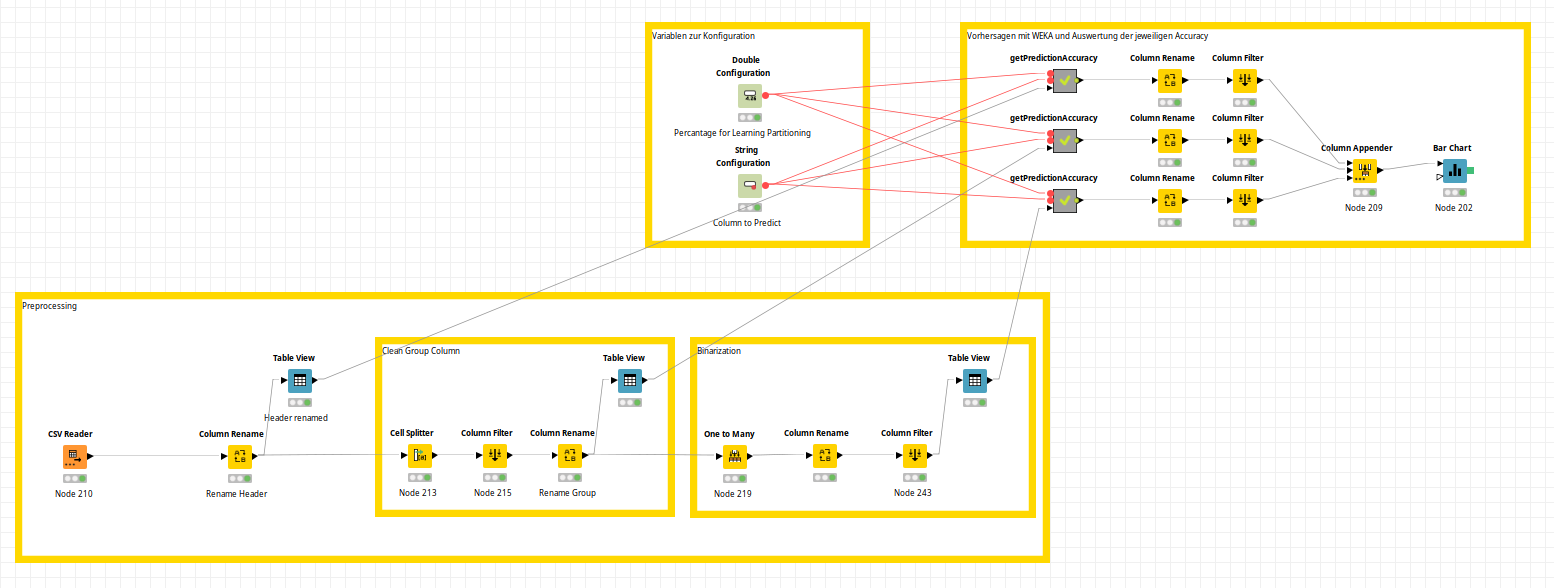
\includegraphics[scale=0.3]{pictures/trees-workflow-gesamt.png}
				\caption{Aufbau des Workflows}									
				\label{figure:trees:workflow}
			\end{center}
		\end{figure}
		
		\begin{figure}[h]
			\begin{center}
				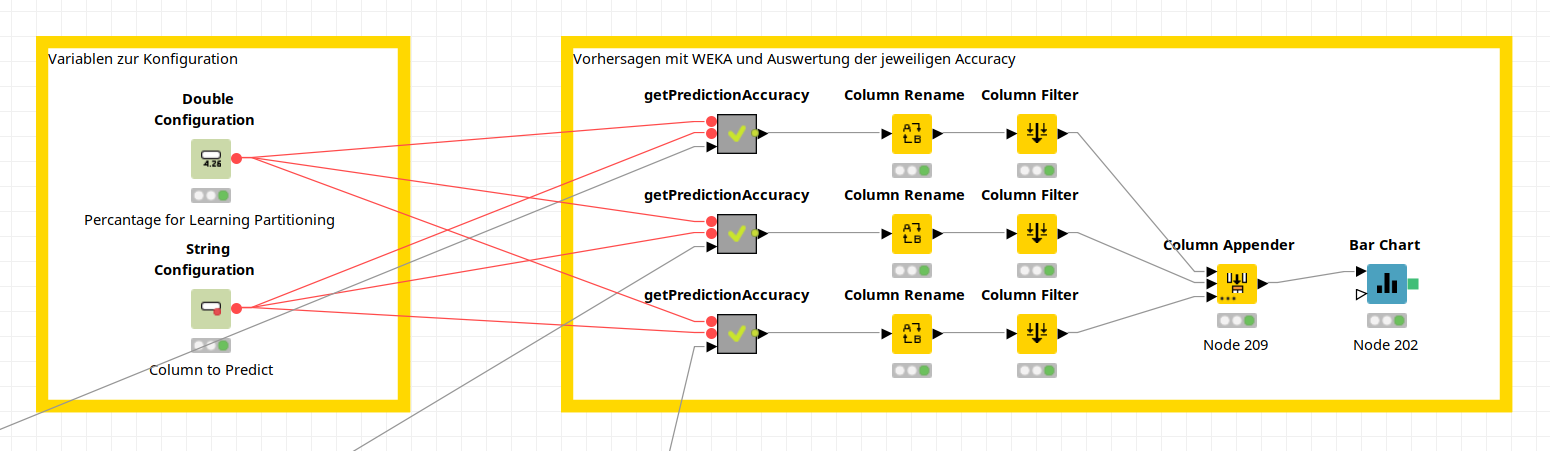
\includegraphics[scale=0.3]{pictures/trees-workflow-gesamt-zoomed.png}
				\caption{Ausschnitt des Workflows (Variableneingabe und Vorhersage)}									
				\label{figure:trees:workflow:zommed}
			\end{center}
		\end{figure}
		
		\begin{figure}[h]
			\begin{center}
				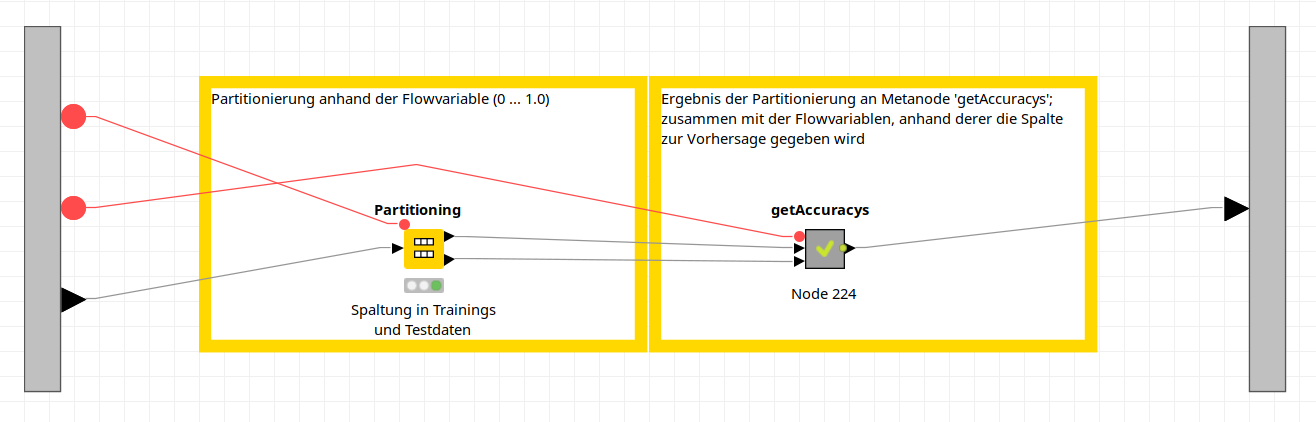
\includegraphics[scale=0.35]{pictures/trees-workflow-partitioning.png}
				\caption{Inhalt des Metanodes `getPredictionAccuracy'}									
				\label{figure:trees:workflow:partitioning}
			\end{center}
		\end{figure}
		
		Hierbei wird dem Metaknoten `getPredictionAccuracy' dreimal der verschieden aufbereitete Datensatz übergeben. Von ihm ausgegeben werden, die Werte des `Accuracy' Feldes für jeden in Kapitel \ref{tree:dec:nodes} genannten Entscheidungsbaum-Knoten. Die Trainingsmengen sind hierbei immer gleich (vgl. Abblidung \ref{figure:trees:workflow:partitioning}). Zusammengefügt und visualisiert werden die Ergebnisse in einem Barchart.
		
		Der in Abbildung \ref{figure:trees:workflow:partitioning}	 gezeigte Metaknoten `getAccuracys' ist in Abbildung \ref{figure:trees:workflow:getaccuracys} genauer dargestellt. Er beinhaltet für jeden in Kapitel \ref{tree:dec:nodes} genannten Entscheidungsbaum einen eigenen Metaknoten dessen Inhalt analog zu dem in Abbildung \ref{figure:trees:workflow:example:weka} ist. Übergeben werden hierbei die Trainings und die Testmenge, sowie der Name der vorherzusagende Spalte. Der Knoten `Scorer' erzeugt unteranderem den zu vergleichenden Wert `Accuracy', welcher durch einen Spalten- und Reihenfilter extrahiert und umbenannt wird.
		
		\begin{figure}[h]
			\begin{center}
				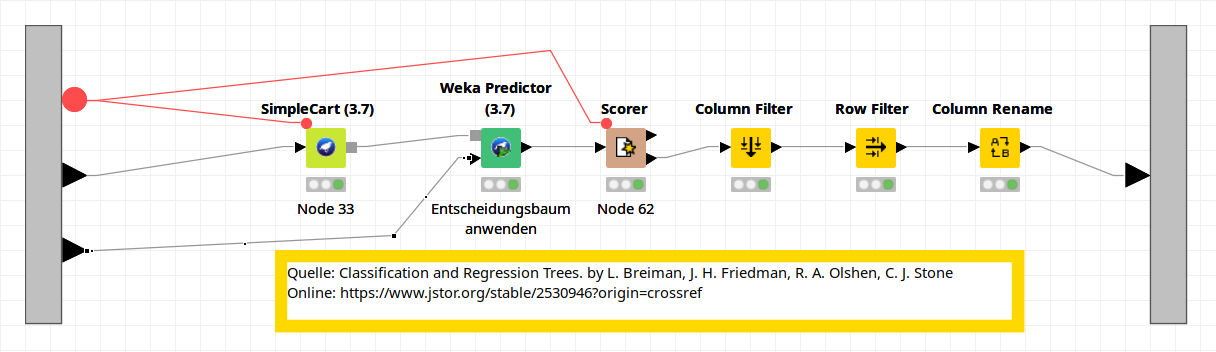
\includegraphics[scale=0.35]{pictures/trees-workflow-weka-example.png}
				\caption{Inhalt des Metanodes `getAccuracyWekaSimpleCart'}									
				\label{figure:trees:workflow:example:weka}
			\end{center}
		\end{figure}
		
		\begin{figure}[h]
			\begin{center}
				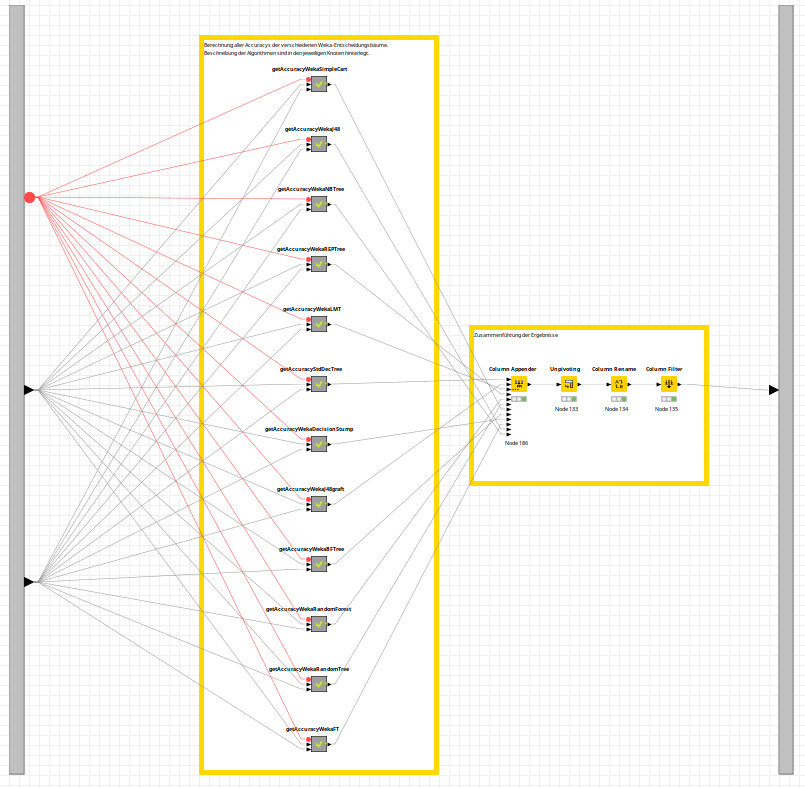
\includegraphics[scale=0.55]{pictures/trees-workflow-getAccuracys.png}
				\caption{Inhalt des Metanodes `getAccuracys'}									
				\label{figure:trees:workflow:getaccuracys}
			\end{center}
		\end{figure}

	\section{Clusteranalyse}
		\subsection{Relevante Knoten}
		\subsection{kMeans Cluster Workflow}
		\subsection{Dichtebasierters Cluster Workflow}
		\subsection{Hierarchisches Cluster Workflow}
	%-----------------------------------------------------------------------------
	% Literaturverzeichnis einf�gen, 
	% Nutzung der BibTeX-Technologie --> literatur.bib 
	%-----------------------------------------------------------------------------

	
	\bibliographystyle{unsrtdin}		%  Stil des Literaturverzeichnisses (hier nach DIN 1505)
	\bibliography{literature}			% gibt Datei mit der Literatur an
	
	\nocite{*}						% damit alle in der DB enthaltende Eintr�ge bearbeitet werden
	

	%-----------------------------------------------------------------------------
	% Verzeichnisse
	%-----------------------------------------------------------------------------
	\listoffigures						% Bildverzeichnis einf�gen

	%-----------------------------------------------------------------------------
	% Anhang
	%-----------------------------------------------------------------------------	
	\appendix
	% Auch hier sind Gliederungen aller \chapter, \section
	

	%-----------------------------------------------------------------------------
	% Selbstst�ndigkeitserkl�rung
	%-----------------------------------------------------------------------------	
%	\chapter*{Selbstst\"andigkeitserkl\"arung}
%	\addcontentsline{toc}{chapter}{Selbstst\"andigkeitserkl\"arung}
%	\rhead{Selbstst\"andigkeitserkl\"arung} % rechts oben in der Kopfzeile Chapter darstellen
%	Hiermit erkl\"are ich, dass ich die hier vorliegende Arbeit selbstst\"andig,
%	ohne unerlaubte fremde Hilfe und nur unter Verwendung der aufgef\"uhrten
%	Hilfsmittel angefertigt haben.
%
%	\begin{tabular}{p{10cm}p{13cm}}
%		\\
  %		\\
  	%	\\
 % 		\\
 % 		Wismar, den \today \\
 % 		---------------------------------------  & ------------------------ \\
 % 		Ort, Datum & Unterschrift
%	\end{tabular}
	


\end{document}							% Ende des Dokuments
%-----------------------------------------------------------------------------
